% Options for packages loaded elsewhere
\PassOptionsToPackage{unicode}{hyperref}
\PassOptionsToPackage{hyphens}{url}
\PassOptionsToPackage{dvipsnames,svgnames,x11names}{xcolor}
\PassOptionsToPackage{space}{xeCJK}
\documentclass[
  10pt,
]{article}
\usepackage{xcolor}
\usepackage[margin=0.70in]{geometry}
\usepackage{amsmath,amssymb}
\setcounter{secnumdepth}{-\maxdimen} % remove section numbering
\usepackage{iftex}
\ifPDFTeX
  \usepackage[T1]{fontenc}
  \usepackage[utf8]{inputenc}
  \usepackage{textcomp} % provide euro and other symbols
\else % if luatex or xetex
  \usepackage{unicode-math} % this also loads fontspec
  \defaultfontfeatures{Scale=MatchLowercase}
  \defaultfontfeatures[\rmfamily]{Ligatures=TeX,Scale=1}
\fi
\usepackage{lmodern}
\ifPDFTeX\else
  % xetex/luatex font selection
  \setmainfont[]{Cambria}
  \setmonofont[]{Consolas}
  \ifXeTeX
    \usepackage{xeCJK}
    \setCJKmainfont[]{Microsoft YaHei}
  \fi
  \ifLuaTeX
    \usepackage[]{luatexja-fontspec}
    \setmainjfont[]{Microsoft YaHei}
  \fi
\fi
% Use upquote if available, for straight quotes in verbatim environments
\IfFileExists{upquote.sty}{\usepackage{upquote}}{}
\IfFileExists{microtype.sty}{% use microtype if available
  \usepackage[]{microtype}
  \UseMicrotypeSet[protrusion]{basicmath} % disable protrusion for tt fonts
}{}
\makeatletter
\@ifundefined{KOMAClassName}{% if non-KOMA class
  \IfFileExists{parskip.sty}{%
    \usepackage{parskip}
  }{% else
    \setlength{\parindent}{0pt}
    \setlength{\parskip}{6pt plus 2pt minus 1pt}}
}{% if KOMA class
  \KOMAoptions{parskip=half}}
\makeatother
\usepackage{longtable,booktabs,array}
\newcounter{none} % for unnumbered tables
\usepackage{calc} % for calculating minipage widths
% Correct order of tables after \paragraph or \subparagraph
\usepackage{etoolbox}
\makeatletter
\patchcmd\longtable{\par}{\if@noskipsec\mbox{}\fi\par}{}{}
\makeatother
% Allow footnotes in longtable head/foot
\IfFileExists{footnotehyper.sty}{\usepackage{footnotehyper}}{\usepackage{footnote}}
\makesavenoteenv{longtable}
\usepackage{graphicx}
\makeatletter
\newsavebox\pandoc@box
\newcommand*\pandocbounded[1]{% scales image to fit in text height/width
  \sbox\pandoc@box{#1}%
  \Gscale@div\@tempa{\textheight}{\dimexpr\ht\pandoc@box+\dp\pandoc@box\relax}%
  \Gscale@div\@tempb{\linewidth}{\wd\pandoc@box}%
  \ifdim\@tempb\p@<\@tempa\p@\let\@tempa\@tempb\fi% select the smaller of both
  \ifdim\@tempa\p@<\p@\scalebox{\@tempa}{\usebox\pandoc@box}%
  \else\usebox{\pandoc@box}%
  \fi%
}
% Set default figure placement to htbp
\def\fps@figure{htbp}
\makeatother
\setlength{\emergencystretch}{3em} % prevent overfull lines
\providecommand{\tightlist}{%
  \setlength{\itemsep}{0pt}\setlength{\parskip}{0pt}}
\usepackage{bookmark}
\IfFileExists{xurl.sty}{\usepackage{xurl}}{} % add URL line breaks if available
\urlstyle{same}
\hypersetup{
  colorlinks=true,
  linkcolor={Maroon},
  filecolor={Maroon},
  citecolor={Blue},
  urlcolor={Blue},
  pdfcreator={LaTeX via pandoc}}

\author{}
\date{}

\setlength{\textfloatsep}{10pt plus 2pt minus 2pt}
\renewcommand{\figurename}{图}
\begin{document}

\section{同眼照片标定的眼底退化训练与复核评估}\label{ux540cux773cux7167ux7247ux6807ux5b9aux7684ux773cux5e95ux9000ux5316ux8badux7ec3ux4e0eux590dux6838ux8bc4ux4f30}

Eye Sentinel · 2026 年 11 月 18 日 ·
\href{calibrated-defocus.en.md}{English} ·
\href{calibrated-defocus.zh.pdf}{PDF}

\textbf{同眼标定失焦让模型在轻失焦下的排序表现下降得更少。}
三组配对训练后，AIROGS 开发原图的 AUROC 从 \textbf{0.9687 升至
0.9713}。在 3.2\% 转诊阳性、10\%
复核的情景下，每千张留在复核名单外的误报从 \textbf{18.3 降至
11.0}，漏诊从 \textbf{2.35 到
2.26}，漏诊差值的区间包含零。下文箭头均从原混合指向同眼标定失焦。

\subsection{训练怎样配对}\label{ux8badux7ec3ux600eux6837ux914dux5bf9}

{\def\LTcaptype{none} % do not increment counter
\begin{longtable}[]{@{}ll@{}}
\toprule\noalign{}
条件 & 固定设置 \\
\midrule\noalign{}
\endhead
\bottomrule\noalign{}
\endlastfoot
疾病模型 & EfficientNet-B0，输入为 320 × 320 像素眼底图 \\
训练与模型验证 & 15,480 张训练图；2,046 张模型验证图 \\
比较时间点 & 三个既定随机种子，每种方案比较第 1,200 次参数更新的权重 \\
原混合退化 & 约半数训练抽样施加退化，照明、失焦、散射三类等概率 \\
同眼标定失焦 & 沿用原抽样；只替换原来抽到失焦时的图像处理 \\
\end{longtable}
}

原失焦用随机高斯模糊并加噪声或 JPEG 压缩。同眼标定失焦根据 60 对 Real
Fundus
照片拟合的参数，施加模糊和曝光变化。因为二者一起变化，本轮比较的是整套失焦处理。按
512 像素视野换算，标定模糊的中位半径为 1.7 像素，曝光倍率中位数为
0.99。三种子抽到失焦的次数依次为 3,292 / 3,228 /
3,306。每个种子的逐图抽样次数、来源和类别、各退化类型次数均与对照完全一致。

\begin{figure}
\centering
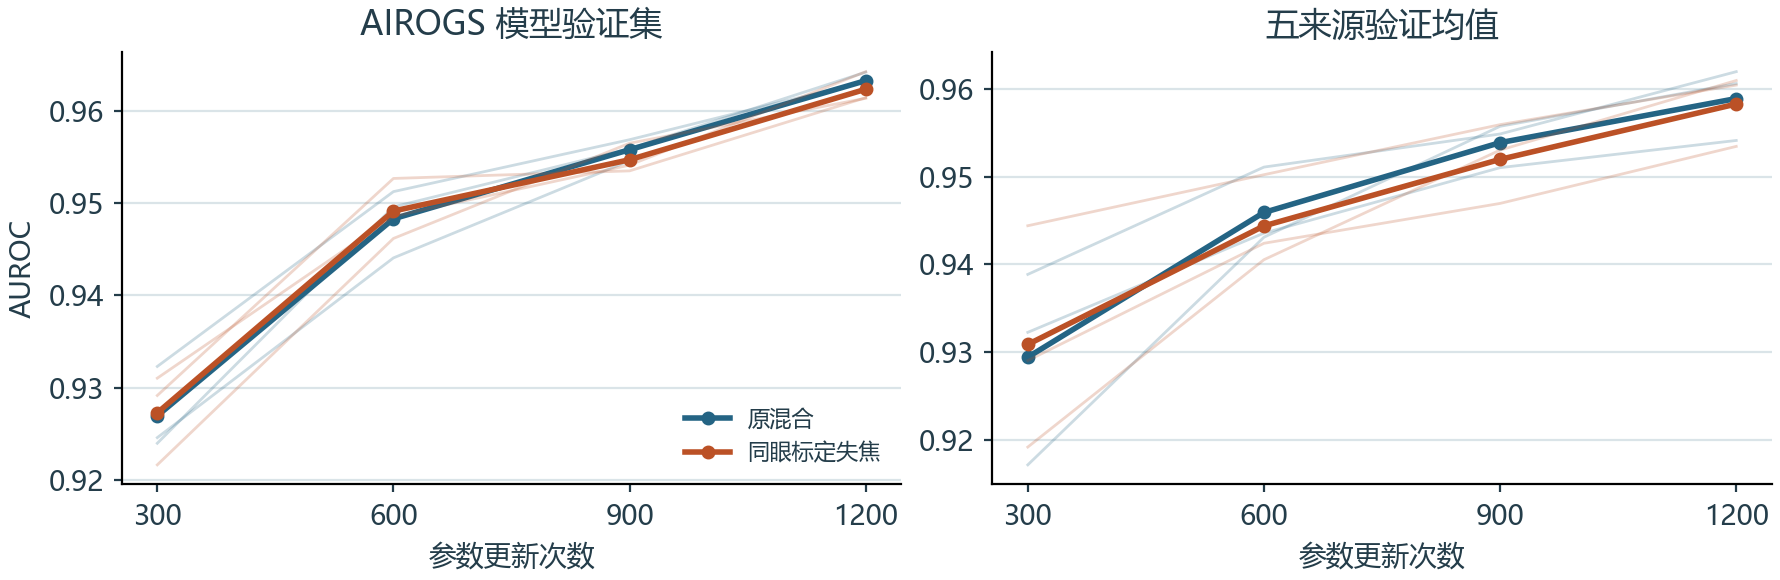
\includegraphics[width=0.98\linewidth,height=\textheight,keepaspectratio,alt={每条细线对应一个随机种子，粗线为三个种子的均值。右图等权平均 AIROGS、ODIR、Kaggle、LAG、KEH 的模型验证 AUROC。}]{calibrated-validation.zh.png}
\caption{每条细线对应一个随机种子，粗线为三个种子的均值。右图等权平均
AIROGS、ODIR、Kaggle、LAG、KEH 的模型验证 AUROC。}
\end{figure}

\textbf{AUROC}
衡量分数排序，等于随机抽一张阳性和一张阴性时，阳性分数排在前面的概率，同分计一半。每
300 次更新记录一次。本轮按预定的第 1,200
次更新比较，开发集用于评估方案，预留独立测试集仍封存。
\href{../../../data/prepared/expanded_20261113/README.md}{冻结数据说明}
·
\href{../../../configs/calibrated_defocus_20261118/profile.json}{标定参数}
· \href{../../../tools/run_calibrated_defocus_20261118.py}{训练脚本} ·
\href{../../../tools/evaluate_calibrated_defocus_20261118.py}{评估脚本}

\newpage

\subsection{原图、模拟失焦和真实低质量图}\label{ux539fux56feux6a21ux62dfux5931ux7126ux548cux771fux5b9eux4f4eux8d28ux91cfux56fe}

{\def\LTcaptype{none} % do not increment counter
\begin{longtable}[]{@{}lrrr@{}}
\toprule\noalign{}
开发图条件 & 图像数 & 原混合 AUROC & 同眼标定失焦 AUROC \\
\midrule\noalign{}
\endhead
\bottomrule\noalign{}
\endlastfoot
全部开发原图 & 2,053 & 0.9716 & 0.9731 \\
AIROGS 开发原图 & 773 & 0.9687 & 0.9713 \\
失焦子集的原图 & 384 & 0.9755 & 0.9777 \\
轻失焦 & 384 & 0.9496 & 0.9669 \\
强失焦 & 384 & 0.9000 & 0.9115 \\
\end{longtable}
}

\begin{figure}
\centering
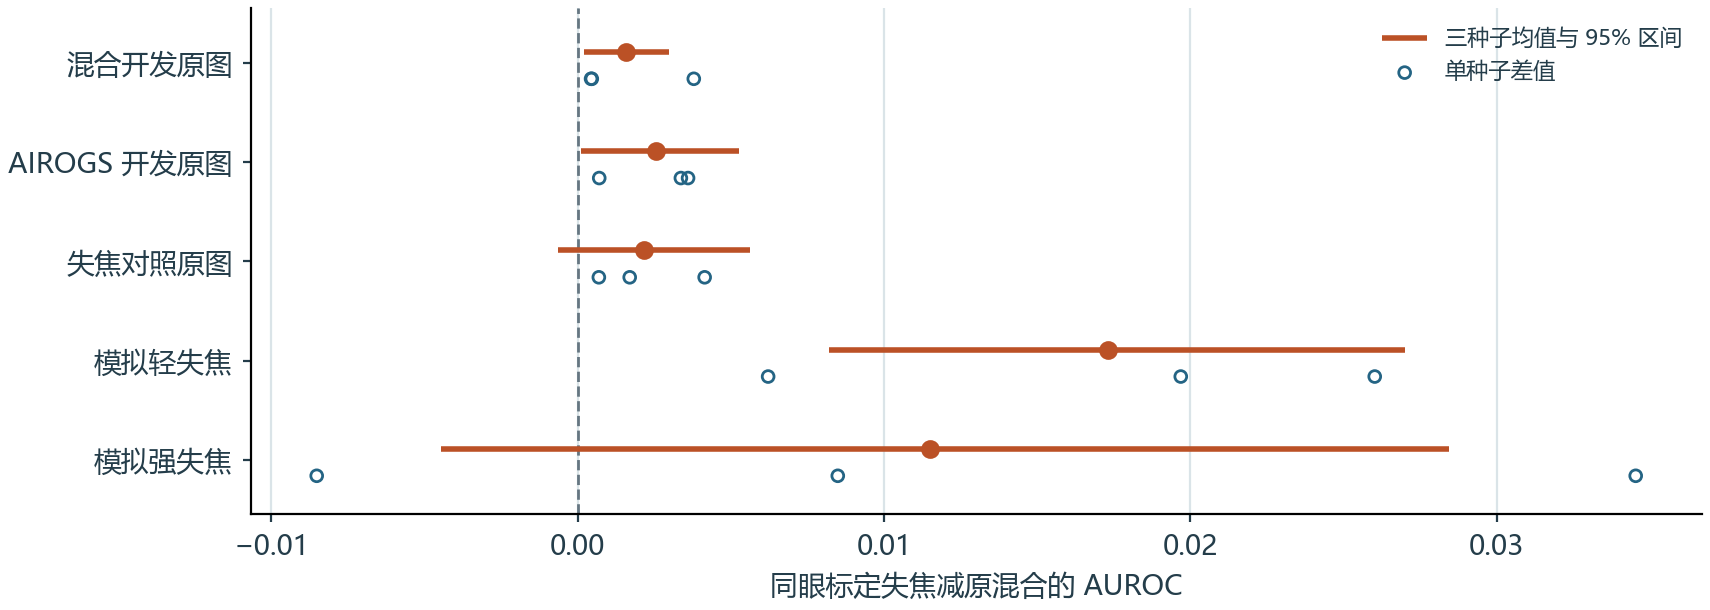
\includegraphics[width=0.98\linewidth,height=\textheight,keepaspectratio,alt={空心点对应三个种子各自的 AUROC 差值，实心点为均值，横线为 95\% 区间。右侧表示同眼标定失焦排序更好。}]{calibrated-development-auroc.zh.png}
\caption{空心点对应三个种子各自的 AUROC 差值，实心点为均值，横线为 95\%
区间。右侧表示同眼标定失焦排序更好。}
\end{figure}

同一批 384
张照片分别保留原图并生成两种模拟失焦图。轻、强失焦的高斯模糊半径分别为
512 像素视野下的 2 和 5。比较模糊前后变化后，标定组比原混合组的
\textbf{AUROC 变化差}，轻失焦为 \textbf{+0.0151} {[}+0.0070,
+0.0236{]}，强失焦为 \textbf{+0.0093} {[}-0.0060,
+0.0251{]}。正值表示标定组的降幅较小。区间来自 2,000
次按关联组配对重抽样，固定三个训练种子。关联组把已知同一患者或有关联的照片作为一个抽样单位。

AIROGS
的阳性表示达到青光眼转诊标准。混合开发图和失焦子集还含其他来源，各自沿用原标签，因此这些合并结果用于比较模型行为。

{\def\LTcaptype{none} % do not increment counter
\begin{longtable}[]{@{}
  >{\raggedright\arraybackslash}p{(\linewidth - 6\tabcolsep) * \real{0.2143}}
  >{\raggedleft\arraybackslash}p{(\linewidth - 6\tabcolsep) * \real{0.2857}}
  >{\raggedleft\arraybackslash}p{(\linewidth - 6\tabcolsep) * \real{0.2857}}
  >{\raggedright\arraybackslash}p{(\linewidth - 6\tabcolsep) * \real{0.2143}}@{}}
\toprule\noalign{}
\begin{minipage}[b]{\linewidth}\raggedright
真实原图质量分层
\end{minipage} & \begin{minipage}[b]{\linewidth}\raggedleft
阳性
\end{minipage} & \begin{minipage}[b]{\linewidth}\raggedleft
阴性
\end{minipage} & \begin{minipage}[b]{\linewidth}\raggedright
两方案三种子检出的阳性（分类分数 \textgreater{} 0.5）
\end{minipage} \\
\midrule\noalign{}
\endhead
\bottomrule\noalign{}
\endlastfoot
原数据人工标为低质量 & 12 & 0 & 原混合 12 / 12 / 11 · 标定 12 / 12 /
12 \\
模型质量分低于 0.20 & 29 & 38 & 原混合 25 / 27 / 26 · 标定 24 / 27 /
28 \\
\end{longtable}
}

FIVES 在模糊、照明或低对比度任一维度标差时计入；MSHF
按整体质量标差计入。模型低质量分层是联合 EyeQ 与 FTHNet 的评分低于
0.20。真实人工标注组没有阴性，测不了该组误报率。
\href{https://www.nature.com/articles/s41597-022-01564-3}{FIVES
数据论文} ·
\href{https://www.nature.com/articles/s41597-023-02188-x}{MSHF 数据论文}

\newpage

\subsection{模拟在哪些方面接近实拍}\label{ux6a21ux62dfux5728ux54eaux4e9bux65b9ux9762ux63a5ux8fd1ux5b9eux62cd}

用 60 对 Real Fundus 照片拟合参数，再用另 60
对比较。数据按照片对划分，缺少患者标识。在每对中，以较清晰照片为起点，比较真实较差照片、原混合退化、按作者实现生成的
CoFe 和 ArcNet 退化，以及同眼标定的模糊加曝光。

\begin{figure}
\centering
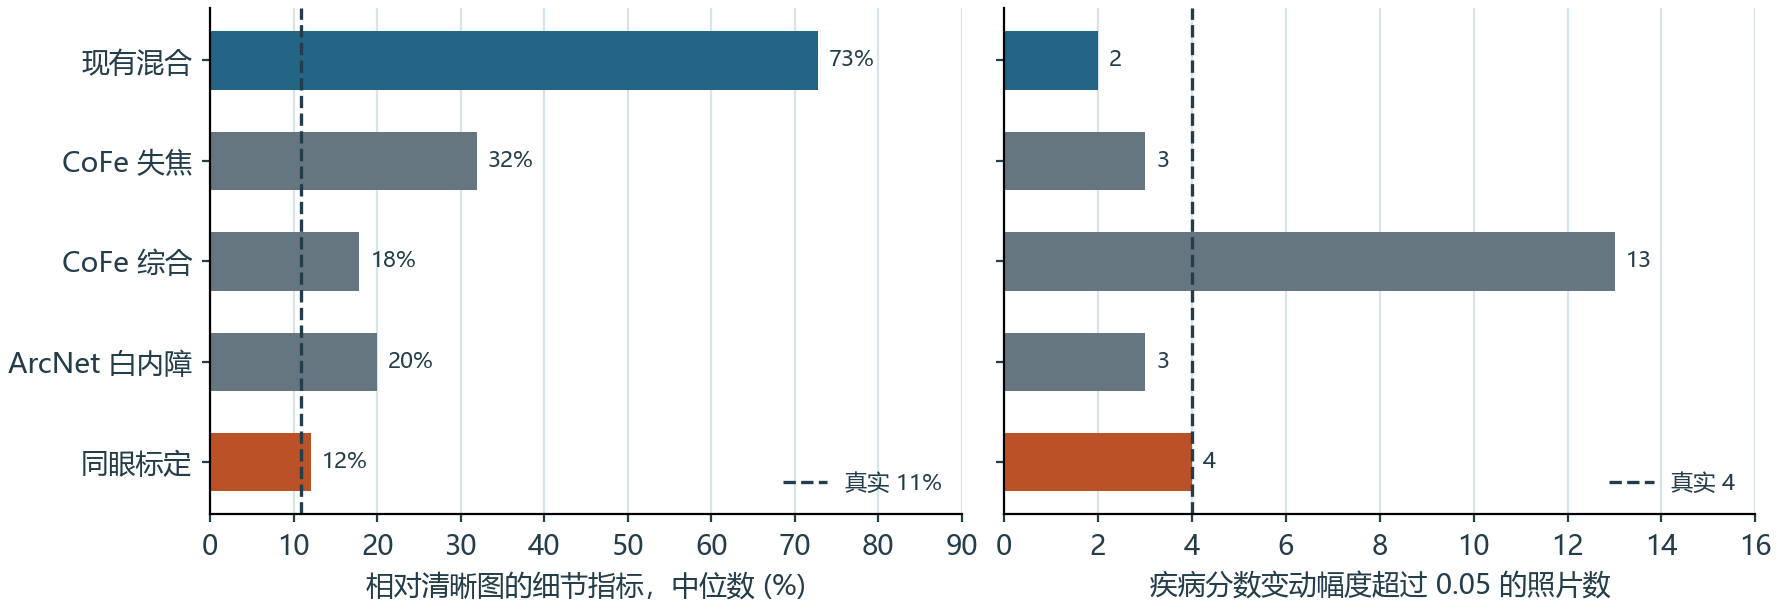
\includegraphics[width=0.98\linewidth,height=\textheight,keepaspectratio,alt={虚线为真实较差照片。左图的细节指标是绿通道拉普拉斯方差比，反映边缘和局部亮度变化。右图比较疾病模型分数变化较大的照片数量，60 张为分母。}]{calibrated-image-benchmark.zh.png}
\caption{虚线为真实较差照片。左图的细节指标是绿通道拉普拉斯方差比，反映边缘和局部亮度变化。右图比较疾病模型分数变化较大的照片数量，60
张为分母。}
\end{figure}

真实较差图的细节指标中位数为同眼较清晰图的 \textbf{11\%}，原混合为
\textbf{73\%}，同眼标定为 \textbf{12\%}。CoFe 综合退化和 ArcNet
白内障模拟分别为 \textbf{18\%} 和
\textbf{20\%}，但平均亮度比实际照片偏暗、偏亮。作者方案能作为不同成像问题的对照。
\href{https://arxiv.org/abs/2201.00466}{Real Fundus} ·
\href{https://arxiv.org/abs/2005.05594}{CoFe-Net} ·
\href{https://arxiv.org/abs/2203.07737}{ArcNet}

同眼标定改善了细节指标的接近程度。用已训练的同一疾病模型比较时，真实较差照片有
\textbf{4/60} 分数变动幅度超过 0.05，原混合为 \textbf{2/60}，同眼标定为
\textbf{4/60}。按分数变化的全分布比较，原混合略近。该照片集提供同眼质量对照，缺少青光眼参考标签。鹿特丹人群研究对
100 张不可判读照片的抽查中，98
张视盘取景不全。下一轮应记录视盘是否完整入镜。
\href{https://www.aaojournal.org/article/S0161-6420\%2826\%2900846-8/fulltext}{真实筛查取景研究}
· \href{review-degradation-benchmark.json}{逐指标结果}

\newpage

\subsection{放回 10\%
复核流程}\label{ux653eux56de-10-ux590dux6838ux6d41ux7a0b}

在 773 张 AIROGS 开发图上，按 \textbf{3.2\%
转诊阳性照片比例}重加权，每千张复核 100
张。每个模型用自己验证集阴性分数的第 95
百分位作分类阈值。灰区优先选分数靠近阈值或质量分数较低的照片。漏诊指参照标签为转诊而模型判阴，误报指参照标签为阴性而模型判转诊。名单外指未进入复核的照片。

\begin{figure}
\centering
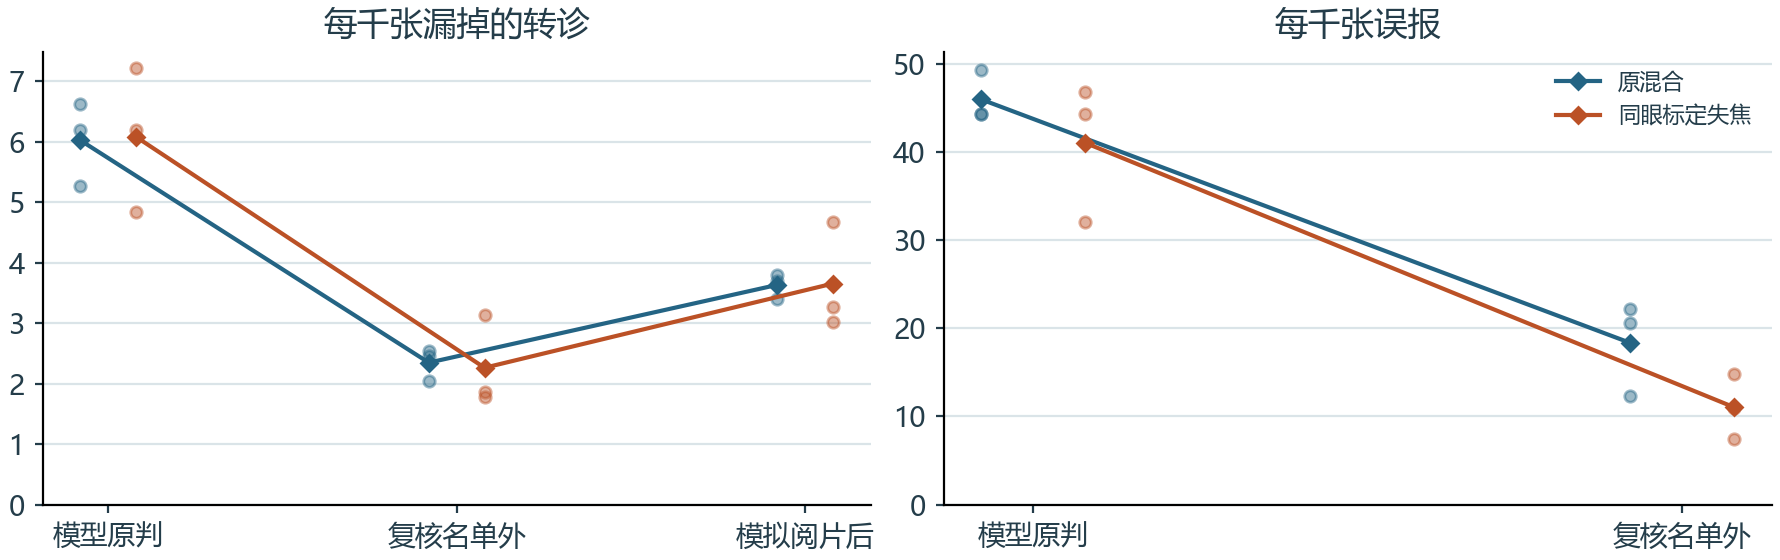
\includegraphics[width=0.92\linewidth,height=\textheight,keepaspectratio,alt={点为各随机种子，菱形为均值。左图最后一项模拟阅片者以 86\% 灵敏度和 96.4\% 特异度接替名单内原判。右图只统计复核分流前后的误报。}]{calibrated-review-routing.zh.png}
\caption{点为各随机种子，菱形为均值。左图最后一项模拟阅片者以 86\%
灵敏度和 96.4\% 特异度接替名单内原判。右图只统计复核分流前后的误报。}
\end{figure}

名单外每千张的漏诊差值为 \textbf{−0.08}，95\% 区间为 {[}−0.47,
+0.40{]}。误报差值为 \textbf{−7.30}，区间为 {[}−14.27,
−1.46{]}。两组分别把 \textbf{60.3\%} 和 \textbf{70.1\%}
的原判错误送入复核。按上述阅片假设，每千张最终仍漏掉 \textbf{3.63 →
3.65} 个转诊。

\begin{figure}
\centering
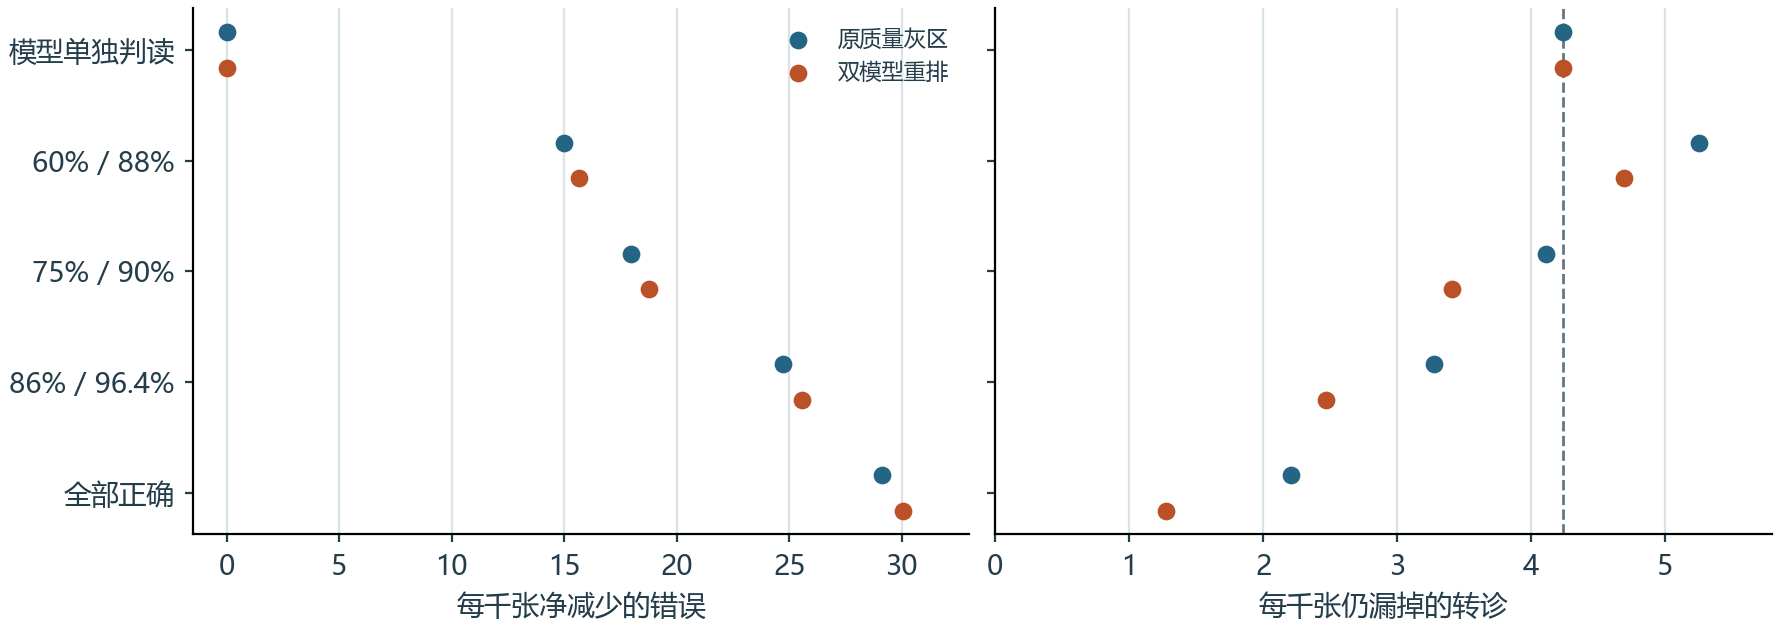
\includegraphics[width=0.92\linewidth,height=\textheight,keepaspectratio,alt={先前第 2,400 次更新的复核比较。纵轴两项百分比分别为阅片灵敏度与特异度，竖线是模型单独判读时的漏诊数。双模型重排是在判阴侧用第二个模型协助安排复核。}]{calibrated-expert-scenarios.zh.png}
\caption{先前第 2,400
次更新的复核比较。纵轴两项百分比分别为阅片灵敏度与特异度，竖线是模型单独判读时的漏诊数。双模型重排是在判阴侧用第二个模型协助安排复核。}
\end{figure}

EyePACS 的受训阅片者灵敏度 86\%、特异度
96.4\%，在图中作为假设用于复核名单。灵敏度表示阳性被正确识别的比例，特异度表示阴性被正确识别的比例。较低阅片灵敏度时，总错误可能减少，漏诊仍可能增加。临床收益还要以患者为单位，用独立参考检查确认最终转诊结果。
\href{https://pubmed.ncbi.nlm.nih.gov/37113471/}{EyePACS 阅片研究} ·
\href{review-failures.zh.md}{此前双模型分析} ·
\href{calibrated-defocus-results.json}{完整汇总和哈希}

\end{document}
